% Chapter 2: Literature Review (revised version, thesis_v2)
\chapter{Literature Review}
\label{chap:relatedwork}

\section{Introduction}

This chapter moves from the general to the specific. Section~\ref{sec:lit-readability} reviews
readability assessment as a research field, from the first formulas to machine learning, deep
learning and transformer models, and ends with the ordinal and ranking losses that readability
research in other languages has used. Section~\ref{sec:lit-arabic} turns to Arabic: what makes
it hard and why methods built for English do not transfer directly.
Section~\ref{sec:lit-prebarec} reviews the Arabic readability projects that came before BAREC,
formulas, feature-based classifiers, lexicons and corpora, and states for each one what it could
not support. Section~\ref{sec:lit-barec} presents BAREC as the answer to those gaps, and
Section~\ref{sec:lit-input} explains the two design choices this thesis inherits from it, the
D3Tok input and the AraBERTv2 encoder. Section~\ref{sec:lit-ordinal} reviews the ordinal
learning methods compared in this thesis, Section~\ref{sec:lit-systems} the systems of the BAREC
2025 Shared Task, and Section~\ref{sec:lit-position} places this thesis among them.

% =====================================================================
\section{Readability Assessment}
\label{sec:lit-readability}

Readability is the ease with which a reader can read and understand a text
\cite{dubay2004principles}. Automatic readability assessment predicts it, usually as a grade or a
level on an ordered scale, and is used to match texts to readers, to build graded reading
material, to evaluate text simplification and to control the difficulty of generated text
\cite{collins2014computational,vajjala2022trends,xu-etal-2015-problems,agrawal2019controlling}.
Early English datasets were drawn from graded textbooks, and later ones from crowdsourced
annotations, simplified news articles and second-language examinations
\cite{vajjala2012readability,xu-etal-2015-problems,xia2016readability,vajjala2022trends}.

\subsection{Traditional Readability Formulas}

Early readability research relied on handcrafted formulas that estimate difficulty from shallow
counts such as sentence length, word length and syllables per word
\cite{dubay2004principles}. The Flesch Reading Ease score \cite{flesch1948readability}, the
Dale--Chall formula \cite{dale1948formula}, the SMOG grade \cite{mclaughlin1969smog} and the
Flesch--Kincaid grade level are the best known. They were developed for English and became
popular because they are simple and cheap to compute.

\begin{table}[H]
\centering
\caption{Examples of traditional readability formulas.}
\label{tab:traditional_readability}
\begin{tabular}{p{3.6cm} p{5.6cm} p{2.2cm}}
\toprule
\textbf{Formula} & \textbf{Main Features} & \textbf{Language} \\
\midrule
Flesch Reading Ease & Sentence length and syllables per word & English \\
Flesch--Kincaid Grade Level & Sentence length and syllables per word & English \\
Dale--Chall & Sentence length and share of unfamiliar words & English \\
SMOG Index & Number of polysyllabic words & English \\
\bottomrule
\end{tabular}
\end{table}

\begin{figure}[H]
\centering
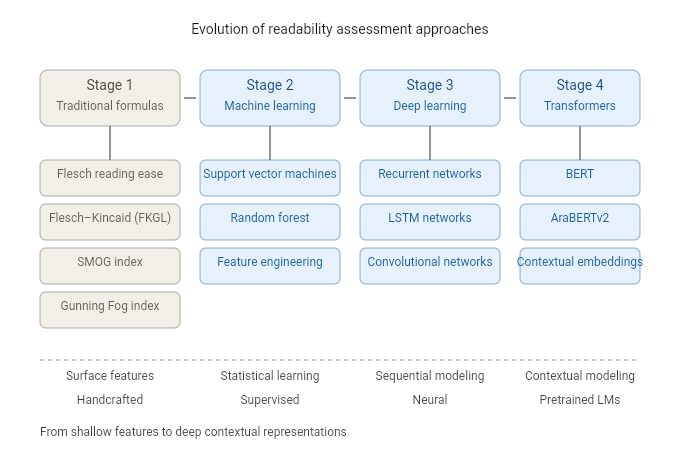
\includegraphics[width=0.98\linewidth]{readability_assessment_evolution@1x.png}
\caption{How readability assessment evolved, from traditional handcrafted formulas to contextual
language models based on transformers.}
\label{fig:evolution}
\end{figure}

These formulas assume that longer sentences and longer words make a text harder. They miss
vocabulary, syntax, discourse and background knowledge, and they cannot tell apart two texts
with the same lengths but very different difficulty. The limitation is sharper for
morphologically rich languages such as Arabic, where a single long word may hold a conjunction,
an article, a stem and a pronoun \cite{habash2010introduction}.

\subsection{Machine Learning Approaches}

Machine learning approaches treat readability as a supervised classification or regression
problem over extracted features. Early systems combined lexical, syntactic and statistical
features, such as word frequency, the distribution of parts of speech, the depth of the parse
tree and language model probabilities, with classifiers such as support vector machines
\cite{schwarm2005reading,collins2004language}. Support vector machines, random forests, logistic
regression and naive Bayes were all widely used, and they improved clearly on the formulas.

\begin{table}[H]
\centering
\caption{Common machine learning methods used for readability assessment.}
\label{tab:ml_readability}
\begin{tabular}{p{3.6cm} p{5.6cm} p{2.2cm}}
\toprule
\textbf{Method} & \textbf{Main Characteristics} & \textbf{Learning Type} \\
\midrule
Support Vector Machines & Margin-based supervised classification & Supervised \\
Random Forest & Ensemble of decision trees & Supervised \\
Logistic Regression & Linear probabilistic classification & Supervised \\
Naive Bayes & Probabilistic feature-based classification & Supervised \\
\bottomrule
\end{tabular}
\end{table}

The BAREC benchmark reports the same family on Arabic: a support vector machine over a count
vectorizer on D3Tok input reaches a QWK of only 56.5\%, and a decision tree 52.5\%
\cite{elmadani2025barec}, far below the pretrained models discussed below.

\subsection{Deep Learning Approaches}

Deep learning removed most of the feature engineering. Recurrent networks, long short-term memory
networks, their bidirectional variants and convolutional networks learn representations directly
from text, and hierarchical attention networks model the structure of sentences and documents
\cite{martinc2021supervised}. They capture sequential dependencies and semantic relations that
hand-crafted features miss, but they need large annotated datasets and considerable computation
when trained from scratch.

\begin{table}[H]
\centering
\caption{Common deep learning architectures used for readability assessment.}
\label{tab:deep_learning_readability}
\begin{tabular}{p{3.6cm} p{5.6cm} p{2.2cm}}
\toprule
\textbf{Architecture} & \textbf{Main Characteristics} & \textbf{Learning Type} \\
\midrule
RNN & Sequential text modelling & Deep Learning \\
LSTM & Long-range dependency modelling & Deep Learning \\
CNN & Local feature extraction & Deep Learning \\
BiLSTM & Bidirectional contextual sequence modelling & Deep Learning \\
\bottomrule
\end{tabular}
\end{table}

\subsection{Transformer-Based Language Models}

Transformer models replaced recurrence with self-attention \cite{vaswani2017attention}, which
lets them relate any two words of a sentence directly and process a sequence in parallel. BERT
\cite{devlin2019bert} pretrains a bidirectional transformer with masked language modelling on
large corpora and is then fine-tuned for the task at hand. Fine-tuned transformers are among the
strongest models for readability assessment \cite{martinc2021supervised}, and Deutsch et al.\
found that adding hand-crafted linguistic features to them gives little further gain
\cite{deutsch2020linguistic}.

\begin{table}[H]
\centering
\caption{Examples of transformer-based language models used in NLP.}
\label{tab:transformer_models}
\begin{tabular}{p{3.6cm} p{5.6cm} p{2.2cm}}
\toprule
\textbf{Model} & \textbf{Main Characteristics} & \textbf{Language} \\
\midrule
BERT & Bidirectional contextual transformer & English \\
RoBERTa & Optimised BERT pretraining & English \\
DistilBERT & Compressed transformer & English \\
AraBERTv2 & BERT pretrained on segmented Arabic & Arabic \\
\bottomrule
\end{tabular}
\end{table}

\subsection{Ordinal and Ranking Losses in Readability Research}
\label{sec:lit-readability-losses}

Readability levels are ordered, and research on English and Chinese readability has increasingly
used losses that respect that order. Lim and Lee compare ordinal log loss, soft labels, the
Earth Mover's Distance and a weighted kappa loss with cross-entropy on English and Chinese
corpora, and find that ordinal log loss improves adjacent accuracy significantly on most of
them \cite{lim-lee-2024-improving}. Zeng et al.\ train with soft labels for ordinal regression
together with a pre-training step that predicts which of two texts is harder
\cite{zeng-etal-2022-enhancing}, and Li et al.\ weight cross-entropy by the length profile of
each level \cite{li-etal-2022-unified}.

A second line of work treats readability as ranking. Lee and Vajjala train a neural pairwise
ranking model that learns which of two texts is harder, and report zero-shot ranking accuracy
above 80 per cent on French and Spanish after training on English \cite{lee2022neural}; their
model is trained with a pairwise logistic loss. Trokhymovych et al.\ score the readability of
Wikipedia articles in 14 languages with a model trained by a margin ranking loss on pairs of
articles and their simplified versions \cite{trokhymovych2024readability}. On the ordinal side,
CORN extends the CORAL framework by removing its shared weights and training each binary
question on a conditional subset of the data \cite{shi2023corn}.

None of these losses was among those evaluated by the BAREC benchmark, and none of the BAREC
2025 system papers that describe their loss reports CORN or a pairwise ranking loss; the ZAI
system paper names CORN explicitly as future work \cite{nazzal2025zai}. They are therefore the natural candidates for
the addition this thesis makes in Chapters~\ref{chap:methodology} and~\ref{chap:results}.

% =====================================================================
\section{Arabic Readability Assessment}
\label{sec:lit-arabic}

Arabic readability is not English readability with different words. Four properties of the
language break the assumptions behind English methods \cite{habash2010introduction,
nassiri2023approaches}.

\begin{enumerate}
\item \textbf{Morphology and clitics.} Words are derived from roots through patterns and carry
attached conjunctions, prepositions, articles and pronouns, so word length and word counts mean
something different from English, and a word-frequency list sees many forms of one lexeme as
different words.
\item \textbf{Missing short vowels.} Most Arabic is written without diacritics, so syllables,
the basic unit of English formulas, cannot be counted from the written text without first
restoring the vowels automatically.
\item \textbf{Ambiguity.} An undiacritized word can have several readings, and choosing the
rarer one requires more knowledge, which is itself a mark of difficulty.
\item \textbf{Diglossia and register.} Modern Standard Arabic coexists with spoken dialects and
with Classical Arabic, so the difficulty of a text depends on vocabulary and constructions from
very different periods and registers.
\end{enumerate}

These properties mean that an Arabic readability model needs either morphological analysis or a
pretrained model that has learned the morphology, and a dataset whose labels reflect the
linguistic phenomena Arabic readers actually find hard. The next section shows how the work
before BAREC approached both needs.

% =====================================================================
\section{Arabic Readability Projects before BAREC}
\label{sec:lit-prebarec}

Arabic readability research before 2025 falls into three groups: formulas adapted from English,
feature-based machine learning, and lexical and corpus resources with models built on them
\cite{nassiri2023approaches,elmadani2025barec}. The subsections below describe each group, and
Table~\ref{tab:lit-prebarec} and Section~\ref{sec:lit-gaps} summarise what they could and could
not support. The limitations stated here are limitations for the purpose of this thesis,
fine-grained sentence-level modelling; most of these projects were designed for a different
purpose and served it well.

\subsection{Readability Formulas for Arabic}

The first Arabic tools followed the English formulas. Al-Khalifa and Al-Ajlan built
\emph{Arability}, a prototype that estimates readability from surface features such as word and
sentence length with statistical models, using reading books collected manually from the
elementary, intermediate and secondary curricula of Saudi schools, that is, three levels
\cite{al2010automatic}. The Automatic Arabic Readability Index (AARI) of Al-Tamimi et al.\ was
fitted by factor analysis on 1{,}196 texts from the Jordanian curriculum for grades one to ten,
and combines the number of characters, the average word length and the average sentence length
in a single linear formula \cite{altamimi2014aari}.

OSMAN, by El-Haj and Rayson, adapts the Flesch approach to Arabic
\cite{elhaj2016osman}. Because Arabic is usually written without short vowels, it first adds
diacritics automatically with an open-source diacritizer and then counts short, long and stressed
syllables; it also adds a \emph{Faseeh} factor for letters and word endings typical of formal
writing. It was evaluated by correlating its scores over 73{,}000 parallel English and Arabic
sentences from United Nations documents.

These formulas share the weaknesses of their English models and add some of their own. They use
surface counts that ignore morphology, syntax and vocabulary, which are exactly the dimensions
along which Arabic difficulty varies. They were calibrated on the school curriculum of one
country, so their scale is the grade system of that curriculum. OSMAN's syllable counts depend on
the accuracy of an automatic diacritizer, and its evaluation goes through the parallel English
sentences rather than through levels assigned to Arabic text by Arabic readers. None of them produces
a fine-grained level that can be checked against expert labels at sentence level.

\subsection{Feature-Based Machine Learning}

Saddiki et al.\ studied 146 features, from average word length to the depth of the syntactic
parse tree, for Arabic as a first and as a second language \cite{saddiki2018feature}. On a
first-language corpus of 27{,}688 texts in four levels their best model reaches 94.8 per cent
accuracy, and on the second-language task 72.4 per cent. Khallaf and Sharoff classified the
difficulty of Modern Standard Arabic sentences for language learners, either on a three-way scale
derived from the Common European Framework of Reference (CEFR) or as simple against complex
\cite{khallaf2021automatic}. They compared sentence embeddings from fastText, multilingual BERT,
XLM-R and an Arabic BERT with traditional features, and obtained their best result, an F1 of
0.80 on the three-way task and 0.94 on the binary task, with the fine-tuned Arabic BERT.

These studies showed that learned models beat formulas and that pretrained Arabic encoders help,
but their high scores are obtained on coarse scales of two to four levels, where a large share of
the task is separating very easy from very hard text. The first works on whole texts, not
sentences, and the second on a learner scale collapsed to three classes. Neither scale can
express the difference between, say, a text for the second and one for the third school grade.

\subsection{Lexical Resources and Corpora}

The SAMER project took a lexical route. Its readability lexicon assigns one of five levels to
about 26{,}000 lemmas of Modern Standard Arabic, each annotated in triplicate by language
professionals from three regions of the Arab world \cite{alkhalil2020samer}. It led to the SAMER
simplification corpus, the first manually annotated Arabic parallel corpus for text
simplification: 159{,}000 words from 15 Arabic novels, most of them published between 1865 and
1955, each simplified by hand to two lower levels \cite{alhafni2024samer}. In that corpus the
level of a text is defined as the highest level of any of its words. Liberato et al.\ used it to
model readability at the level of words and of text fragments, combining frequency, rule-based
and pretrained models, and reached a macro F1 of 86.7 at word level and 87.9 at fragment level on
a blind test set \cite{liberato2024strategies}.

DARES collects 13{,}335 texts from the Saudi school textbooks of 2021, with a coarse task that
predicts the educational stage and a fine task that predicts the school grade
\cite{elhaj2024dares}. ReadMe++ annotates 9{,}757 sentences in Arabic, English, French, Hindi and
Russian from 112 sources and 21 domains on the six CEFR levels \cite{naous2024readme}, so Arabic
is one of five languages in it.

Each resource answered a real need, and each carries a limitation for fine-grained modelling.
The SAMER lexicon rates words out of context, and the SAMER corpus inherits that view: a sentence
is as hard as its hardest word, whatever its syntax, and the texts are nineteenth- and
early-twentieth-century fiction. DARES labels a text with the grade of the textbook it came from,
which is a property of where the text was published rather than a judgement of the text itself,
and it covers one country's curriculum in one year. ReadMe++ uses a second-language scale of six
levels, built for comparison across languages rather than for the Arabic school system.

\subsection{Summary of the Projects}

\begin{table}[H]
\centering
\footnotesize
\caption{Arabic readability work before BAREC. The last column states the main limitation for
fine-grained, sentence-level modelling, which is not always the purpose the work was designed
for.}
\label{tab:lit-prebarec}
\setlength{\tabcolsep}{3pt}
\begin{tabular}{p{2.3cm} p{0.8cm} p{1.3cm} p{1.7cm} p{2.4cm} p{2.9cm}}
\toprule
\textbf{Work} & \textbf{Year} & \textbf{Unit} & \textbf{Scale} & \textbf{Data} &
\textbf{Main limitation} \\
\midrule
Arability \cite{al2010automatic} & 2010 & text & 3 levels & Saudi school reading books &
surface features, one curriculum \\
AARI \cite{altamimi2014aari} & 2014 & text & grades 1--10 & 1{,}196 Jordanian curriculum texts &
linear formula of length counts \\
OSMAN \cite{elhaj2016osman} & 2016 & text & continuous score & 73{,}000 UN sentence pairs &
depends on automatic diacritization; validated through English \\
Saddiki et al.\ \cite{saddiki2018feature} & 2018 & text & 4 levels & 27{,}688 texts &
coarse scale, heavy feature pipeline \\
SAMER lexicon \cite{alkhalil2020samer} & 2020 & word & 5 levels & about 26{,}000 lemmas &
words out of context \\
Khallaf and Sharoff \cite{khallaf2021automatic} & 2021 & sentence & 3 CEFR levels & learner
sentences & learner scale, coarse \\
SAMER corpus \cite{alhafni2024samer} & 2024 & word, text & 5 levels & 159{,}000 words, 15 novels &
one genre; level = hardest word \\
Liberato et al.\ \cite{liberato2024strategies} & 2024 & word, fragment & SAMER levels & SAMER
corpus & inherits SAMER's lexical definition \\
DARES \cite{elhaj2024dares} & 2024 & text & stages, grades & 13{,}335 textbook texts & label is
the textbook's grade \\
ReadMe++ \cite{naous2024readme} & 2024 & sentence & 6 CEFR levels & 9{,}757 sentences, 5
languages & Arabic is one fifth; L2 scale \\
\bottomrule
\end{tabular}
\end{table}

\subsection{What Was Missing}
\label{sec:lit-gaps}

Read together, the projects leave six gaps for anyone who wants to model fine-grained Arabic
readability and to compare models on it.

\begin{enumerate}
\item \textbf{Granularity.} The scales range from three levels to one level per school grade.
A model evaluated on three levels can be very accurate while being unable to separate adjacent
school grades.
\item \textbf{Unit.} The labels are attached to words or to whole texts. Sentence-level labels,
which let a model be checked against a human judgement for every sentence, exist only in
learner-oriented or multilingual form.
\item \textbf{Source of the label.} Several labels are proxies: the grade of the source
textbook, the hardest word of a text, or the readability of a translation. None is an expert's
judgement of the specific text against explicit linguistic criteria.
\item \textbf{Coverage.} Each resource covers one curriculum, one genre or one learner
population.
\item \textbf{Features.} The formulas and most feature sets use length counts and ignore the
morphology that makes Arabic hard.
\item \textbf{A shared benchmark.} Without one large corpus with fixed public splits and an agreed
metric, results obtained on different datasets cannot be compared.
\end{enumerate}

% =====================================================================
\section{The BAREC Corpus}
\label{sec:lit-barec}

The Balanced Arabic Readability Evaluation Corpus was built to close these gaps
\cite{elmadani2025barec,habash2025guidelines}. Its levels follow the 19-level system of
Taha-Thomure for Arabic children's books \cite{tahathomure2017}, named in the Abjad order of the
Arabic letters from 1-\textit{alif} to 19-\textit{qaf} and running from kindergarten to
postgraduate comprehension, with finer distinctions at the lower levels where readability varies
most. Through the BAREC pyramid the 19 levels collapse into coarser schemes of 7, 5 and 3 levels,
so one model trained at the finest granularity can be evaluated at any coarser one.

Annotators assign each sentence the level of its most difficult linguistic phenomenon, judged
along six dimensions: spelling, word count, morphology, syntax, vocabulary and content. The
guidelines define which phenomena of each dimension qualify a sentence for a given level; clitics
and infrequent inflections such as the dual, for example, are morphological markers of higher
levels \cite{habash2025guidelines}. The annotation team consisted of six native speakers, all
experienced Arabic language educators, and every sentence of the first phase was checked twice.

The corpus contains 69{,}441 sentences and about one million words from 1{,}922 documents drawn
from 30 resources, organised in three domains (Arts and Humanities, Social Sciences, STEM) and
three readership groups (Foundational, Advanced, Specialized); about a quarter of the sentences
come from sources that were typed by hand to make them digitally usable \cite{elmadani2025barec}.
It is split at the document level into training, development and test sets of 80, 10 and 10 per
cent, so that no document contributes to more than one split.

Agreement between annotators was measured in 16 studies. The average pairwise exact agreement on
the 19 levels is only 61.1 per cent, but the average pairwise QWK is 81.8 per cent and the
average distance 0.94 levels, so most disagreements are between neighbouring levels. Against the
unified labels agreed after discussion, individual annotators reach 71.7 per cent exact agreement
and a QWK of 88.1 per cent \cite{elmadani2025barec}.

\begin{table}[H]
\centering
\caption{Main characteristics of the BAREC corpus \cite{elmadani2025barec}.}
\label{tab:barec_characteristics}
\begin{tabular}{p{4.2cm} p{7.4cm}}
\toprule
\textbf{Characteristic} & \textbf{Description} \\
\midrule
Language & Modern Standard Arabic \\
Size & 69{,}441 sentences, about 1 million words \\
Sources & 1{,}922 documents from 30 resources \\
Domains & Arts and Humanities, Social Sciences, STEM \\
Readership groups & Foundational, Advanced, Specialized \\
Readability levels & 19 ordered levels, collapsible to 7, 5 and 3 \\
Unit of annotation & sentence \\
Annotation & manual, by six expert Arabic educators, over six linguistic dimensions \\
Agreement & 81.8\% pairwise QWK; 88.1\% QWK against the unified label \\
Splits & 80\% train, 10\% development, 10\% test, at document level \\
\bottomrule
\end{tabular}
\end{table}

Table~\ref{tab:lit-gaps-barec} shows how the corpus answers each gap of
Section~\ref{sec:lit-gaps}.

\begin{table}[H]
\centering
\footnotesize
\caption{The gaps left by earlier Arabic readability work and the corresponding property of
BAREC.}
\label{tab:lit-gaps-barec}
\begin{tabular}{p{2.8cm} p{4.0cm} p{4.6cm}}
\toprule
\textbf{Gap} & \textbf{Before BAREC} & \textbf{BAREC} \\
\midrule
Granularity & from 3 levels to one per school grade & 19 levels, collapsible to 7, 5 and 3 \\
Unit & words or whole texts & every sentence labelled \\
Source of the label & textbook grade, hardest word, English side & expert judgement against
explicit criteria in six dimensions \\
Coverage & one curriculum, genre or learner group & 30 resources, 3 domains, 3 readership
groups \\
Measured reliability & rarely reported at sentence level & 16 agreement studies, 81.8\% pairwise
QWK \\
Shared benchmark & different datasets and metrics & fixed document-level splits, QWK, a shared
task \\
\bottomrule
\end{tabular}
\end{table}

The benchmark paper that introduced the corpus also gives the reference results that this thesis
reproduces. The best single model, AraBERTv2 with D3Tok input trained as a regression, reaches
84.4\% QWK on the test set; an average of six models reaches 84.5\%; and an oracle that picks the
best of the six predictions for each sentence reaches 94.7\% \cite{elmadani2025barec}.

% =====================================================================
\section{Input Representation and Encoder}
\label{sec:lit-input}

Two components of the pipeline are chosen once and kept fixed: the form in which a sentence is
given to the model, and the pretrained encoder that reads it. Both follow the evidence in the
BAREC benchmark.

\subsection{D3Tok: Morphological Segmentation}

The corpus provides four input variants of every sentence, produced with the morphological
disambiguator of CAMeL Tools \cite{obeid2020camel,elmadani2025barec}. \emph{Word} is the
tokenised, dediacritized sentence; \emph{Lex} replaces every word by its lemma; \emph{D3Tok}
splits every word into its base and its clitics and marks each clitic boundary with a
\texttt{+}; and \emph{D3Lex} replaces the base of the D3Tok form by its lemma. The written token
\textit{walfi\d{d}\d{d}a} (``and the silver''), for instance, becomes \texttt{w+ Al+ fDp} in
D3Tok, with the conjunction, the article and the noun visible as separate units.

D3Tok is the right choice for readability for two reasons. Linguistically, clitics are among the
features the annotation guidelines use to set a sentence's level \cite{habash2025guidelines}, so
the segmentation shows the encoder the very units the annotators looked at, while keeping the
word forms that Lex and D3Lex discard. Empirically, D3Tok with AraBERTv2 is the best of the
sixteen model and input combinations the benchmark evaluated, as Table~\ref{tab:lit-inputs}
shows.

\subsection{AraBERTv2}

AraBERTv2 \cite{antoun2020arabert} is a BERT-base model (12 layers, 12 attention heads, hidden
size 768) pretrained on about 8.6 billion words of Arabic. What sets it apart from the other
Arabic encoders is its pretraining data: the text was segmented with the Farasa segmenter
\cite{darwish2016farasa}, which also separates clitics from their host word and marks the
boundaries with \texttt{+}. D3Tok input therefore matches the distribution AraBERTv2 saw during
pretraining, which is not true of any other encoder in the comparison.

\begin{figure}[H]
\centering
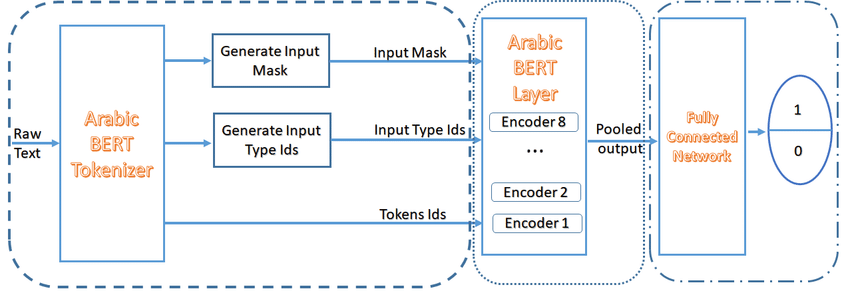
\includegraphics[width=0.79\linewidth]{Arabic-BERT-model-architecture.png}
\caption{General architecture of transformer-based Arabic language models such as AraBERTv2.}
\label{fig:arabert_arch}
\end{figure}

Table~\ref{tab:lit-inputs} reproduces the evidence from the benchmark paper. AraBERTv2 is the
only encoder that improves when the input is segmented: its QWK rises from 76.3\% with word
input to 80.0\% with D3Tok, while the three other encoders lose between 0.2 and 1.0 points. The
benchmark therefore carries AraBERTv2 with D3Tok into its comparison of loss functions, and this
thesis does the same so that its reproduction of that comparison is meaningful.

\begin{table}[H]
\centering
\footnotesize
\caption{Development-set QWK (\%) of four Arabic encoders on the four input variants, all trained
with cross-entropy, as reported in Table~5 of the BAREC benchmark \cite{elmadani2025barec}. The
best value is in bold.}
\label{tab:lit-inputs}
\begin{tabular}{lrrrr}
\toprule
\textbf{Encoder} & \textbf{Word} & \textbf{Lex} & \textbf{D3Tok} & \textbf{D3Lex} \\
\midrule
CamelBERT-msa & 79.1 & 77.1 & 78.2 & 78.0 \\
MARBERTv2 & 79.1 & 77.0 & 78.9 & 78.0 \\
AraBERTv02 & 79.2 & 78.5 & 78.2 & 78.2 \\
AraBERTv2 & 76.3 & 77.7 & \textbf{80.0} & 78.6 \\
\bottomrule
\end{tabular}
\end{table}

% =====================================================================
\section{Ordinal Regression and Distance-Aware Learning}
\label{sec:lit-ordinal}

Ordinal regression is the family of methods for labels with a natural order
\cite{gutierrez2016ordinal}. Where classification treats the classes as unrelated, ordinal
methods take the distance between them into account, which suits readability: predicting level
10 instead of 11 should cost less than predicting level 1 instead of 11.

\begin{table}[H]
\centering
\footnotesize
\caption{Ordinal-aware learning methods compared in this thesis.}
\label{tab:ordinal_methods}
\begin{tabular}{p{3.2cm} p{5.8cm} p{2.4cm}}
\toprule
\textbf{Method} & \textbf{Main Characteristics} & \textbf{Paradigm} \\
\midrule
Cross-Entropy (CE) & Classification without ordinal awareness & Classification \\
Regression (MSE) & Continuous prediction with a squared-error loss & Regression \\
CORAL & $K{-}1$ binary questions with one shared projection & Ordinal regression \\
CORN & $K{-}1$ conditional binary questions, no shared weights & Ordinal regression \\
Ordinal Log Loss (OLL) & Distance-weighted penalty on wrong levels & Ordinal classification \\
Earth Mover's Distance (EMD) & Squared difference of cumulative distributions & Ordinal
classification \\
Soft labels (SOFT) & Targets that decay with distance & Ordinal classification \\
Soft-QWK & Differentiable surrogate of the QWK metric & Metric optimisation \\
Pairwise ranking (RANK, PLR) & Regression plus a penalty on mis-ordered pairs & Learning to rank
\\
\bottomrule
\end{tabular}
\end{table}

CORAL models the ordinal prediction as a sequence of $K{-}1$ binary questions ``is the level
greater than $k$?'' that share one projection and differ only in their bias, so the ordering is
built into the output \cite{cao2020coral}. CORN keeps the $K{-}1$ questions but gives each its own
weights and trains question $k$ only on the examples above level $k-1$, recovering the
probabilities by the chain rule \cite{shi2023corn}. Ordinal log loss weights the probability
given to each wrong level by its distance from the true level \cite{castagnos2022ordinal}; the
soft-label loss replaces the one-hot target by one that decays with distance
\cite{bertinetto2020soft}; and the Earth Mover's Distance loss compares cumulative distributions
\cite{hou2017emd}. The Soft-QWK loss optimises a differentiable surrogate of QWK
\cite{delatorre2018wkl,diaz2019softlabels}; because that surrogate is a statistic of the whole
batch, it can be lowered by predicting near the mean level, and the STBW system therefore
precedes it with a mean squared error warm-up \cite{trigui2025stbw}. The pairwise ranking losses
of Section~\ref{sec:lit-readability-losses} add a penalty whenever a harder text is scored below
an easier one, either with a hinge \cite{trokhymovych2024readability} or with a logistic function
\cite{lee2022neural,burges2005learning}.

% =====================================================================
\section{Systems Developed for the BAREC Shared Task}
\label{sec:lit-systems}

The BAREC 2025 Shared Task on Arabic readability assessment was organised at the Third Arabic
Natural Language Processing Conference (ArabicNLP 2025) \cite{elmadani2025sharedtask}. It
attracted 22 registered teams from 12 countries, and 17 of them submitted system description
papers. It defined two subtasks, at sentence level and at document level, and three resource
tracks, Strict, Constrained and Open, with QWK on a blind test set as the official ranking
metric.

The most successful systems combined D3Tok segmentation with Arabic pretrained encoders,
ordinal-aware losses and ensembling. Large language models and less standard architectures such
as graph neural networks and vision--language models generally did worse than the transformer
baselines, and only five teams went above the strongest baseline of the organisers (AraBERTv2 with
D3Tok and regression, 84.6\% blind QWK).

Two systems are especially relevant to this thesis. The ZAI system used AraBERTv2 with a CORAL
head trained with a binary cross-entropy summed over the $K{-}1$ thresholds; it selected its
checkpoint by QWK, stopped early with a patience of two epochs and tuned a single decision
threshold on the development set, reaching 85.5\% QWK on the blind test set \cite{nazzal2025zai}.
Its paper names alternative ordinal objectives such as CORN as future work. The STBW system used
AraBERTv2 with a single-output regression head and a two-phase schedule, a mean squared error
warm-up followed by a differentiable Soft-QWK objective, which raised its own test QWK from 83.9\%
to 84.88\% and reached 85.6\% on the blind test set; besides the segmented sentence, its input
carries corpus metadata and surface statistics \cite{trigui2025stbw}. These two systems are the
reason both CORAL and Soft-QWK are included in the present comparison, and because their
protocols differ, this thesis reimplements both inside one fixed pipeline instead of comparing
published numbers.

Table~\ref{tab:barec_systems} summarises the benchmark, the baselines of the organisers and the
participating systems, with their approaches and their sentence-level QWK.

\begin{table}[H]
\centering
\footnotesize
\caption{Work on the BAREC dataset: corpus benchmark, organiser baselines, and BAREC 2025 Shared
Task systems (sentence level, Strict track). QWK is the primary metric; higher is better.}
\label{tab:barec_systems}
\begin{tabular}{p{2.3cm} p{0.8cm} p{4.3cm} p{2.2cm} p{1.1cm}}
\toprule
\textbf{Team / Source} & \textbf{Year} & \textbf{Model / Approach} & \textbf{Loss / Method} &
\textbf{QWK (\%)} \\
\midrule
\multicolumn{5}{l}{\textit{Corpus benchmark (Elmadani et al., 2025), test set}} \\
\midrule
BAREC best single & 2025 & AraBERTv2 + D3Tok & Regression (MSE) & 84.4 \\
BAREC ensemble & 2025 & Average of 6 AraBERTv2 models & Ensemble & 84.5 \\
BAREC oracle & 2025 & Best of 6 per sentence & Oracle & 94.7 \\
SVM baseline & 2025 & SVM, count vectorizer, D3Tok & Classification & 56.5 \\
\midrule
\multicolumn{5}{l}{\textit{Organiser baselines, blind test set}} \\
\midrule
Baseline III & 2025 & AraBERTv2 + D3Tok & Regression & 84.6 \\
Baseline II & 2025 & AraBERTv2 + D3Tok & CE & 81.5 \\
Baseline I & 2025 & AraBERTv02 + Word & CE & 80.5 \\
\midrule
\multicolumn{5}{l}{\textit{Shared Task systems, blind test set (Strict track, sentence level)}}
\\
\midrule
!MSA & 2025 & Ensemble of 4 Arabic PLMs + LLM augmentation & CE + OLL + MSE + ordinal &
\textbf{87.5} \\
AMAR & 2025 & Stacked meta-learner over 7 transformers & Regression + meta-classifier & 86.4 \\
mucAI & 2025 & AraBERTv2 + conformal prediction & CE / EMD / Focal & 85.7 \\
STBW & 2025 & AraBERTv2, two-phase training & MSE $\rightarrow$ Soft-QWK & 85.6 \\
ZAI & 2025 & AraBERTv2 + CORAL ordinal head & CORAL (BCE) & 85.5* \\
Syntaxa & 2025 & AraBERTv2 + dependency-graph GNN & GNN & 84.3 \\
MorphoArabia & 2025 & Morphology-aware regression & Regression & 84.2 \\
MARSAD & 2025 & Specialised AraBERT, two-stage & CE $\rightarrow$ WKL & 84.1 \\
Noor & 2025 & Hybrid transformer + features & PLM + features & 83.1 \\
Phantoms & 2025 & Hybrid BERT + linguistic features & PLM + features & 82.7 \\
Qais & 2025 & Fine-tuned PLM (+ LLM) & Classification & 82.5 \\
LIS & 2025 & Curriculum learning with PLMs & Curriculum & 82.4 \\
SATLab & 2025 & Character and token $n$-grams (non-neural) & ML & 82.3 \\
PalNLP & 2025 & Ordinal regression + $K$-fold ensemble & Ordinal regression & 81.1 \\
GNNinjas & 2025 & Lexicon-enriched graph modelling & GNN & 78.5 \\
ANLPers & 2025 & Neural classifiers on embeddings & Neural classifier & 73.0* \\
Pixel & 2025 & Vision--language rendered-text model & VLM & 66.2 \\
\bottomrule
\end{tabular}

\vspace{0.15cm}
{\footnotesize * Trained on the development set; not strictly comparable to the other systems.}
\end{table}

% =====================================================================
\section{Positioning of This Thesis}
\label{sec:lit-position}

This thesis has a different aim from the shared-task systems. It does not try to maximise the
leaderboard through ensembling, data augmentation or external resources. It isolates the effect
of the prediction head and the loss function on one fixed AraBERTv2 and D3Tok pipeline, with
every other component kept at the value the benchmark script sets, and it adds to the
benchmark's losses three kinds of objective that the benchmark does not evaluate: the ordinal
heads used by the strongest systems (CORAL and the two-phase Soft-QWK schedule), the successor of
CORAL that one of those systems names as future work (CORN), and the pairwise ranking losses of
readability research in other languages. Every one of them is compared with a matched control
under the same protocol, so that a difference in the results can be attributed to the loss.

\section{Summary}

This chapter traced readability assessment from formulas based on sentence and word length to
transformer models, and showed that research on English and other languages has moved towards
losses that respect the order of the levels or treat readability as ranking. It then described
what makes Arabic different and reviewed the Arabic work before BAREC: formulas such as
Arability, AARI and OSMAN; feature-based classifiers such as those of Saddiki et al.\ and Khallaf
and Sharoff; and resources such as the SAMER lexicon and corpus, DARES and ReadMe++. Each of them
worked on coarse scales, on words or whole texts, on one curriculum, genre or learner population,
or with labels that are proxies for difficulty. BAREC answers these gaps with 69{,}441
expert-labelled sentences on 19 levels, fixed splits and measured agreement, and its benchmark
shows why AraBERTv2 with D3Tok input is the right fixed backbone. The chapter ended with the
ordinal learning methods and the shared-task systems that this thesis builds on, and with the
position of this thesis among them.

\textit{The next chapter presents the methodology: the corpus and its splits, the D3Tok input, the
encoder and the prediction heads, the exact form of every loss function including the three added
ones, the initialisation of the CORAL cut-points, the training protocol with its declared
differences from the published script, and the evaluation setup.}
